
\section{Diferenças} % (fold)
\label{sec:diferen_as}

\begin{frame}
\begin{figure}[p]
    \centering
    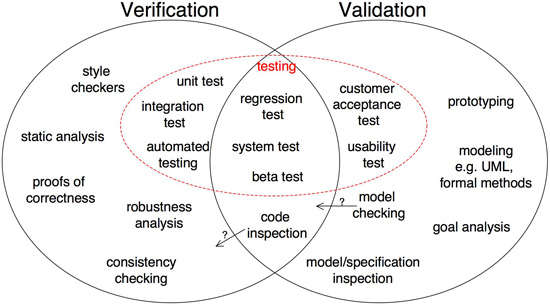
\includegraphics[width=0.8\textwidth]{conteudo/VandVtoolbox.jpg}
    \caption{\href{http://www.easterbrook.ca/steve/2010/11/the-difference-between-verification-and-validation/}{Easterbrook, Steve - Novembro de 2010}}	
    \label{fig:Pattern}
\end{figure}
\end{frame}
% section diferen_as (end)

\section{Verificação} % (fold)
\label{sec:verifica_o}

\begin{frame}
\begin{figure}[p]
    \centering
    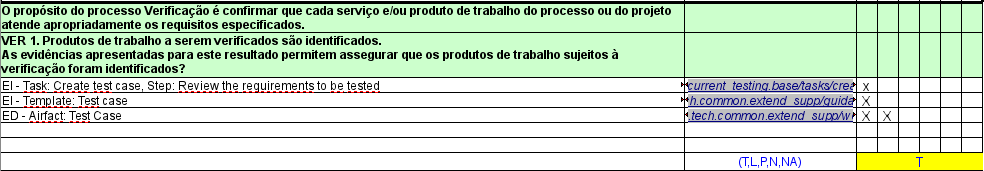
\includegraphics[width=\textwidth]{conteudo/VER1-uc}
    \label{fig:Pattern}
\end{figure}	
\end{frame}
\begin{frame}
\begin{figure}[p]
    \centering
    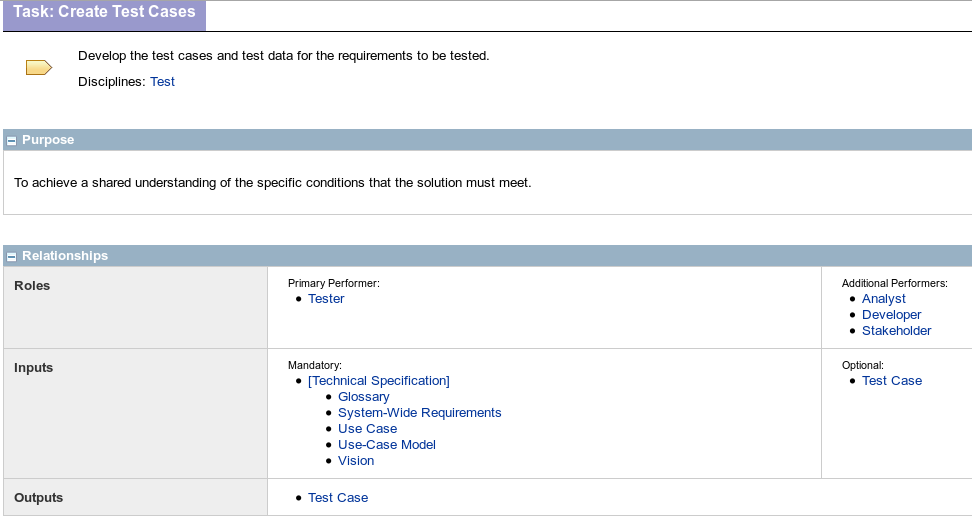
\includegraphics[width=\textwidth]{conteudo/task-uc}
    \label{fig:Pattern}
\end{figure}	
\end{frame}


\begin{frame}
\begin{figure}[p]
    \centering
    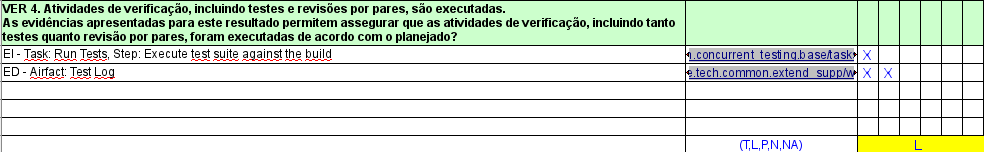
\includegraphics[width=\textwidth]{conteudo/VER4-run_tests}
    \label{fig:Pattern}
\end{figure}	
\end{frame}
\begin{frame}
\begin{figure}[p]
    \centering
    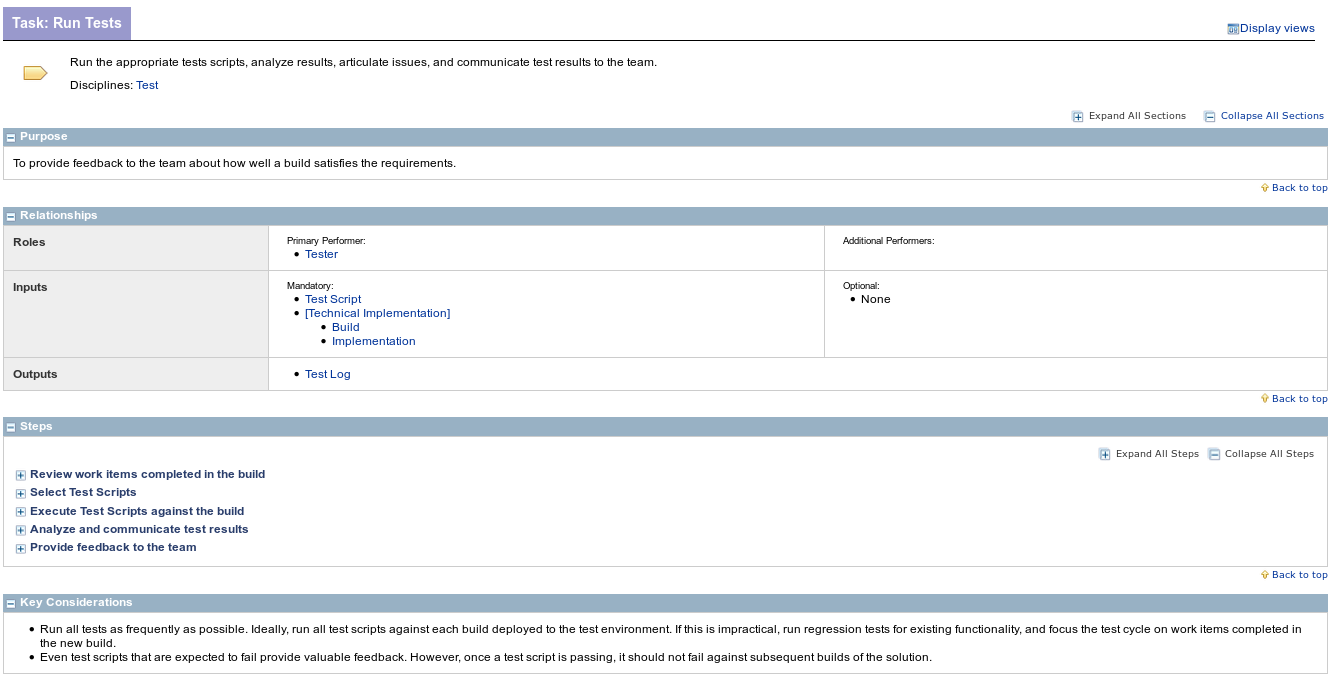
\includegraphics[width=\textwidth]{conteudo/task-run_tests}
    \label{fig:Pattern}
\end{figure}	
\begin{quote}
Sem revisões por pares.
\end{quote}
\end{frame}


\begin{frame}
\begin{figure}[p]
    \centering
    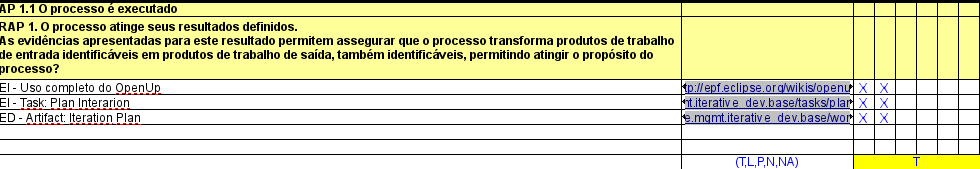
\includegraphics[width=\textwidth]{conteudo/RAP1}
    \label{fig:Pattern}
\end{figure}	
\end{frame}
\begin{frame}
\begin{figure}[p]
    \centering
    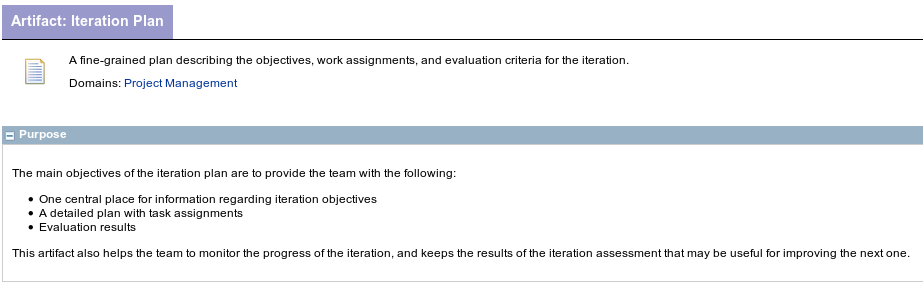
\includegraphics[width=\textwidth]{conteudo/plan}
    \label{fig:Pattern}
\end{figure}	
\begin{quote}
\end{quote}
\end{frame}
% section verifica_o (end)

\section{Validação} % (fold)
\label{sec:valida_o}

\begin{frame}
\begin{figure}[p]
    \centering
    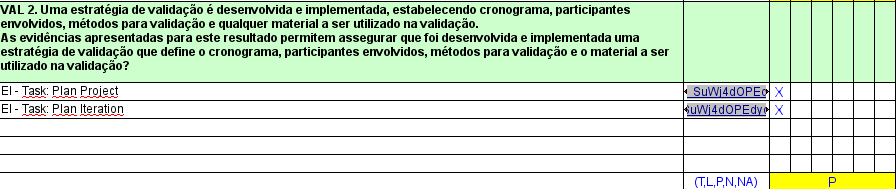
\includegraphics[width=\textwidth]{conteudo/VAL2}
    \label{fig:Pattern}
\end{figure}	
\end{frame}
\begin{frame}
\begin{figure}[p]
    \centering
    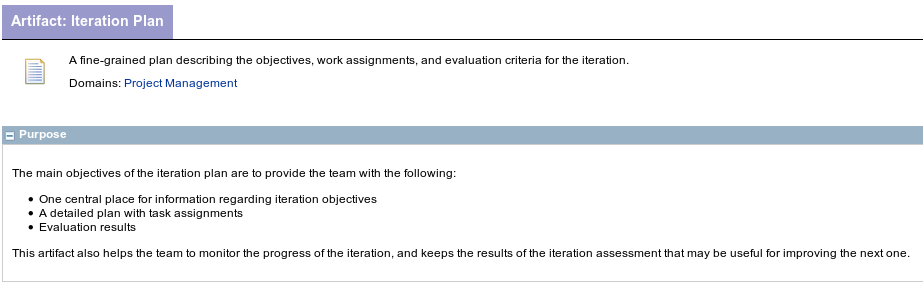
\includegraphics[width=\textwidth]{conteudo/plan}
    \label{fig:Pattern}
\end{figure}	
\begin{quote}
Ausência de previsão de métodos e material de validação previstos.
\end{quote}
\end{frame}


\begin{frame}
\begin{figure}[p]
    \centering
    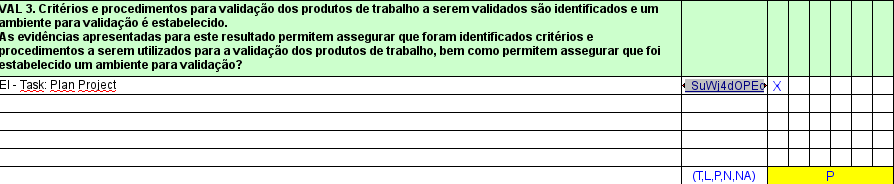
\includegraphics[width=\textwidth]{conteudo/VAL3}
    \label{fig:Pattern}
\end{figure}	
\end{frame}
\begin{frame}
\begin{figure}[p]
    \centering
    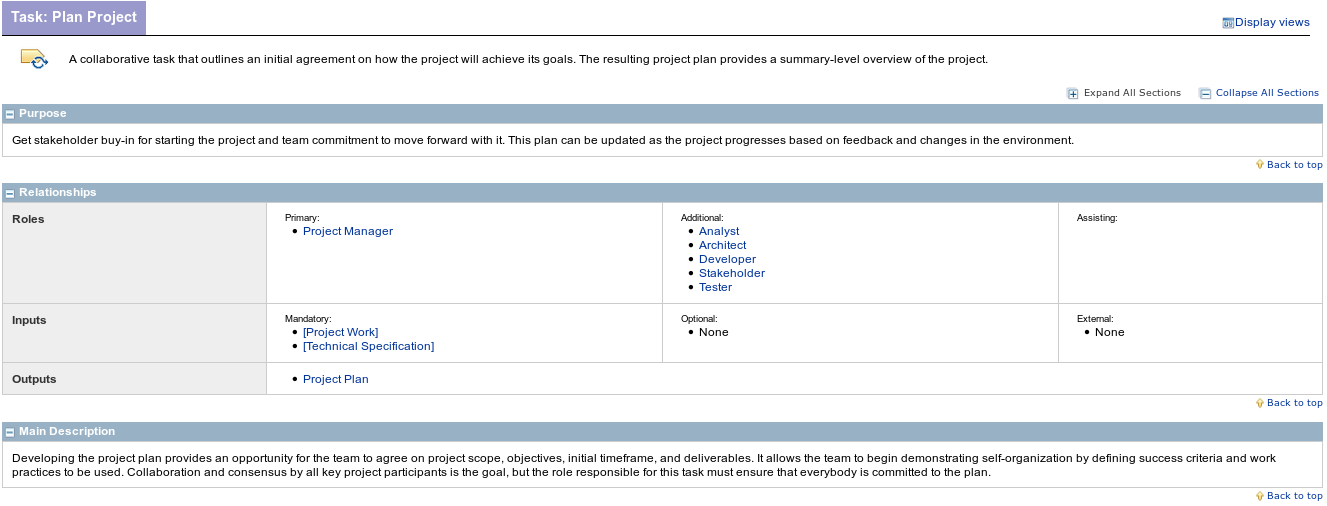
\includegraphics[width=\textwidth]{conteudo/plan2}
    \label{fig:Pattern}
\end{figure}	
\begin{quote}
Apenas critérios são planejados para validação do produto.
\end{quote}
\end{frame}


% section valida_o (end)